\documentclass{article}

\usepackage{amsmath} 
\usepackage{hyperref}
\usepackage[utf8]{inputenc}
\usepackage{graphicx}
\usepackage{array}
\usepackage{indentfirst}
\usepackage{booktabs}
\usepackage[table]{xcolor} 
\usepackage{tikz}
\usepackage{caption}
\usepackage{listings}
\usepackage{xcolor}
\usepackage[utf8]{inputenc}
\usepackage{float}
\usepackage{textcomp}

\lstdefinelanguage{ReduxAsm}{
  keywords={brzr, ji, ld, st, addi, inc, loadv, addv, not, and, or, xor, add, sub, slr, srr},
  morecomment=[l]{;},
  sensitive=true
}

\lstset{
  language=ReduxAsm,
  basicstyle=\ttfamily\small,
  keywordstyle=\color{blue}\bfseries,
  commentstyle=\color{gray},
  frame=single,
  columns=fullflexible
}

\usetikzlibrary{matrix}

\DeclareMathAlphabet{\mathcal}{OMS}{cmsy}{m}{n}
\SetMathAlphabet{\mathcal}{bold}{OMS}{cmsy}{b}{n}
\title{Trabalho 3 - VLIW e Vetorial}
\author{SERGIO SIVONEI DE SANT'ANA FILHO GRR20242337\\EDUARDO KALUF GRR20241770}
\date{\today} 


\begin{document}
    \maketitle
    
    \section{Apresentação}
    
    Ao decorrer da disciplina aprendemos inúmeras maneiras de realizar a implementação de um processador, o modo como operam, seus prós e contras e seus contextos históricos. Sendo assim, neste trabalho iremos nos aprofundar em duas dessas maneiras sendo elas o VLIW e o processador Vetorial, o objetivo é a partir de uma ISA já predefinida (SAGUI) criar o projeto de ambos os processadores utilizando \href{https://github.com/logisim-evolution/logisim-evolution}{\textbf{Logisim}}, criar duas instruções adicionais para cada ISA e então realizar a execução de um programa assembly em cada um deles.

    Para cada um dos processadores iremos utilizar uma ISA diferente que deriva do SAGUI, no caso do VLIW será o Sagui de rabo longo, já para o vetorial o Sagui em bando, além disso, o programa assembly teste consiste em fazer a soma de dois vetores com 12 posições e guardar os resultados na memória, com todos os vetores alinhados.
    Devido a maneira de como os processadores operam, cada um deles terá um programa Assembly diferente, porém que deverá apresentar o mesmo resultado.

    \section{VLIW}
    
    \subsection{Arquitetura}

    VLIW significa "Very long instruction Word" que se traduz para "palavra de instrução muito grande" e a ideia do processador gira exatamente em torno disso, basicamente, iremos ter uma palavra grande que carrega mais de uma instrução dentro dela, no nosso caso, 4 instruções, dessa forma o processador irá executa-las em paralelo aumentando o IPC total.
    No VLIW a responsabilidade de evitar dependencias e escritas simultaneas ficam completamente na mão do compilador, o qual utiliza diversas técnicas como loop unroling e predicação a fim de diminuir a quantidade de NOPS necessários, fazendo com que o código seja executado de maneira mais otimizada.


    \subsection{ISA}

    A ISA que iremos utilizar para o nosso VLIW é a Sagui de Rabo Longo (SRB) com algumas modificações para operar com predicação.
    A SRB consiste em uma ISA parecida com a REDUX-V, sendo tão compacta e amigável quanto para quem está iniciando no mundo da arquitetura de computadores. 
    Ela possui 8 bits com 4 registradores de propósito geral e será endereçada de palavra a palavra ou seja de 4 em 4 bytes, além de definir 4 "lanes" diferentes, esses "lanes" são os tipos de operação (Branch, aritmética, lógica e etc...) que cada posição da palavra do VLIW poderá realizar. O opcode possui 4 bits, fazendo com que possamos operar 16 instruçoes diferentes, devido as modificações para predicação as instruções serão apresentadas mais a frente já em suas lanes específicas.
    
    Por padrão, os formatos das instruções e as lanes são definidas a seguir:

    \begin{table}[h]
      \captionsetup{labelformat=empty, skip=0pt}
      \caption{\textbf{Formato Padrão 1:} Tipo I}
      \centering
      \rowcolors{1}{white}{green!20} 
      \begin{tabular}{|c|*{8}{c|}}
        \hline
        \rowcolor{green!50}
        \multicolumn{9}{|c|}{\textbf{Tipo I}} \\ \hline
        \textbf{Bits} & 7 & 6 & 5 & 4 & 3 & 2 & 1 & 0 \\ \hline
        & \multicolumn{4}{c|}{\textbf{Opcode}} & \multicolumn{4}{c|}{\textbf{Imm.}} \\ \hline
      \end{tabular}
    \end{table}

    \begin{table}[h]
      \captionsetup{labelformat=empty, skip=0pt}
      \caption{\textbf{Formato Padrão 2:} Tipo R}
      \centering
      \rowcolors{1}{white}{blue!20} 
      \begin{tabular}{|c|*{8}{c|}}
        \hline
        \rowcolor{blue!50}
        \multicolumn{9}{|c|}{\textbf{Tipo R}} \\ \hline
        \textbf{Bits} & 7 & 6 & 5 & 4 & 3 & 2 & 1 & 0 \\ \hline
        & \multicolumn{4}{c|}{\textbf{Opcode}} & \multicolumn{2}{c|}{\textbf{Ra}} & \multicolumn{2}{c|}{\textbf{Rb}} \\ \hline
      \end{tabular}
    \end{table}

    \begin{figure}[H]
        \captionsetup{labelformat=empty, skip=0pt}
        \caption{\textbf{Lanes:}}
        \centering 
        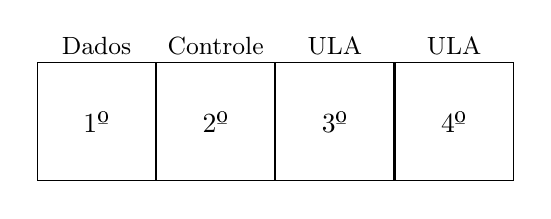
\begin{tikzpicture}
            \matrix[matrix of nodes, 
                    nodes in empty cells,
                    nodes={draw, minimum size=1.5cm, anchor=center},
                    column sep=0pt] (m) {
            {\text{1º}} & {\text{2º}} & {\text{3º}} & {\text{4º}} \\
            };

            \node[yshift=6pt] at (m-1-1.north) {\small Dados};
            \node[yshift=6pt] at (m-1-2.north) {\small Controle};
            \node[yshift=6pt] at (m-1-3.north) {\small ULA};
            \node[yshift=6pt] at (m-1-4.north) {\small ULA};
        \end{tikzpicture}
    \end{figure}

    \subsection{Motivações e Instruções}

    Para este processador gostariamos de dar a maior quantidade de operações lógicas possíveis ao programador e uma facilidade maior para mexer com loops, adicionando outra instrução branch de controle. Além disso, para que a utilização de predicados seja viável, adaptamos a ISA de modo que ela possua um conjunto de instruções específicas para cada uma das lanes do VLIW e instruções para settar o predicado na parte de controle

    \subsubsection{Multi Operations}

    A primeira escolha de instrução foi a de 'multioperações' (MULTIOPS), a qual é do tipo misto (INC) tendo um
    registrador indicado e um imediato de 0 a 3.

    Essa instrução funciona como um grupo de 4 instruções simples, sendo elas: NOT(logico), XOR, AND e XNOR. Todos
    operando sobre R0 (que é sempre o registrador destino) e Ra (por Ra entenda registrador descrito na instrução).

    Ela segue o formato OPCODE nos 4 últimos bits e nos outros 4 ela divide em metade para indicar o
    Ra e outra para um numero de 0 a 3, o qual indica qual operação deve ser realizada, NOT(0), XOR(1),
    AND(2) e XNOR(3).


    \begin{table}[h]
      \captionsetup{labelformat=empty, skip=0pt}
      \caption{\textbf{Formato Novo:} Tipo Misto}
      \centering
      \rowcolors{1}{white}{red!20} 
      \begin{tabular}{|c|*{8}{c|}}
        \hline
        \rowcolor{red!50}
        \multicolumn{9}{|c|}{\textbf{Tipo INC}} \\ \hline
        \textbf{Bits} & 7 & 6 & 5 & 4 & 3 & 2 & 1 & 0 \\ \hline
        & \multicolumn{4}{c|}{\textbf{Opcode}} & \multicolumn{2}{c|}{\textbf{Ra}} & \multicolumn{2}{c|}{\textbf{Imm Unsigned}} \\ \hline
      \end{tabular}
    \end{table}

    \subsubsection{Move}

    A instrução move faz uso da logica de copiar o valor de um registrador para outro, coisa que é 
    útil em casos com grande limitação (como no nosso caso). Isso se dá por, por exemplo, só podermos alterar
    diretamente o valor de R0 (usando as funções movh/movl).
    Essa função faz Ra receber Rb, sobrescrevendo o conteudo anterior de Ra. Tal lógica retira a necessidade de
    zerar um registrador para depois somar por exemplo.

    \subsubsection{Predicação}

    A fim de aproveitar que temos 16 instruções disponíveis por LANE, fizemos a implementação de um sistema de predicados em nosso processador.
    Temos 4 instruções responsáveis por controlar o valor do predicado (TRUE ou FALSE) e então todas as outras instruções possuem um espelho de si mesmas, a primeira funcionando quando o predicado é true e a segunda quando o mesmo é falso.
    Dessa forma o programador pode fazer o caminho verdadeiro de um if junto com o caminho falso, diminuindo a quantidade de dependencias no código.
    Vale a pena resaltar que uma das instruções é o STRUE, a ideia é que ela seja utilizada em conjunto com as instruções que executam o caminho verdadeiro quando nenhuma predicação está acontecendo, assim evitamos criar um terceiro espelho de cada instrução que funcione independente do valor do predicado
    As 4 instruçoes estão apresentadas abaixo juntamente com a tabela final de cada uma das LANES    

    \begin{table}[H]
      \centering
      \captionsetup{labelformat=empty, skip=0pt}
      \caption{\textbf{Lane 1 Instruções: Dados}}
      \rowcolors{1}{white}{gray!20} 
      \begin{tabular}{|c|*{4}{c|}}
        \hline
        \rowcolor{gray!50}
        \multicolumn{1}{|c|}{\textbf{Opcode}} & \multicolumn{1}{|c|}{\textbf{Tipo}} & \multicolumn{1}{|c|}{\textbf{Mnemonic}} & \multicolumn{1}{|c|}{\textbf{Nome}}        & \multicolumn{1}{|c|}{\textbf{Operação}}                      \\ \hline
        \multicolumn{5}{|c|}{\textbf{Dados}} \\ \hline 
        \multicolumn{1}{|c|}{\textbf{0000}}   & \multicolumn{1}{c|}{\textbf{R}}     & \multicolumn{1}{c|}{\textbf{ld}}        & \multicolumn{1}{c|}{\textbf{Load}}         & \multicolumn{1}{c|}{\textbf{R[ra] = M[ R[rb] ] if PR}}       \\ \hline
        \multicolumn{1}{|c|}{\textbf{0001}}   & \multicolumn{1}{c|}{\textbf{R}}     & \multicolumn{1}{c|}{\textbf{st}}        & \multicolumn{1}{c|}{\textbf{Store}}        & \multicolumn{1}{c|}{\textbf{M[ R[rb] ] = R[ra] if PR}}       \\ \hline
        \multicolumn{1}{|c|}{\textbf{0010}}   & \multicolumn{1}{c|}{\textbf{I}}     & \multicolumn{1}{c|}{\textbf{movh}}      & \multicolumn{1}{c|}{\textbf{Move High}}    & \multicolumn{1}{c|}{\textbf{R[0] = {Imm, R[0](3:0)} if PR}}  \\ \hline
        \multicolumn{1}{|c|}{\textbf{0011}}   & \multicolumn{1}{c|}{\textbf{I}}     & \multicolumn{1}{c|}{\textbf{movl}}      & \multicolumn{1}{c|}{\textbf{Move Low}}     & \multicolumn{1}{c|}{\textbf{R[0] = {R[0](7:4), Imm} if PR}}  \\ \hline
        \multicolumn{1}{|c|}{\textbf{0100}}   & \multicolumn{1}{c|}{\textbf{R}}     & \multicolumn{1}{c|}{\textbf{f-ld}}      & \multicolumn{1}{c|}{\textbf{!Load}}        & \multicolumn{1}{c|}{\textbf{R[ra] = M[ R[rb] ] if !PR}}      \\ \hline
        \multicolumn{1}{|c|}{\textbf{0101}}   & \multicolumn{1}{c|}{\textbf{R}}     & \multicolumn{1}{c|}{\textbf{f-st}}      & \multicolumn{1}{c|}{\textbf{!Store}}       & \multicolumn{1}{c|}{\textbf{M[ R[rb] ] = R[ra] if !PR}}      \\ \hline
        \multicolumn{1}{|c|}{\textbf{0110}}   & \multicolumn{1}{c|}{\textbf{I}}     & \multicolumn{1}{c|}{\textbf{f-movh}}    & \multicolumn{1}{c|}{\textbf{!Move High}}   & \multicolumn{1}{c|}{\textbf{R[0] = {Imm, R[0](3:0)} if !PR}} \\ \hline
        \multicolumn{1}{|c|}{\textbf{0111}}   & \multicolumn{1}{c|}{\textbf{I}}     & \multicolumn{1}{c|}{\textbf{f-movl}}    & \multicolumn{1}{c|}{\textbf{!Move Low}}    & \multicolumn{1}{c|}{\textbf{R[0] = {R[0](7:4), Imm} if !PR}} \\ \hline
        \multicolumn{1}{|c|}{\textbf{1000}}   & \multicolumn{1}{c|}{\textbf{EMPTY}} & \multicolumn{1}{c|}{\textbf{EMPTY}}     & \multicolumn{1}{c|}{\textbf{EMPTY}}        & \multicolumn{1}{c|}{\textbf{EMPTY}}                          \\ \hline
        \multicolumn{1}{|c|}{\textbf{1001}}   & \multicolumn{1}{c|}{\textbf{EMPTY}} & \multicolumn{1}{c|}{\textbf{EMPTY}}     & \multicolumn{1}{c|}{\textbf{EMPTY}}        & \multicolumn{1}{c|}{\textbf{EMPTY}}                          \\ \hline
        \multicolumn{1}{|c|}{\textbf{1010}}   & \multicolumn{1}{c|}{\textbf{EMPTY}} & \multicolumn{1}{c|}{\textbf{EMPTY}}     & \multicolumn{1}{c|}{\textbf{EMPTY}}        & \multicolumn{1}{c|}{\textbf{EMPTY}}                          \\ \hline
        \multicolumn{1}{|c|}{\textbf{1011}}   & \multicolumn{1}{c|}{\textbf{EMPTY}} & \multicolumn{1}{c|}{\textbf{EMPTY}}     & \multicolumn{1}{c|}{\textbf{EMPTY}}        & \multicolumn{1}{c|}{\textbf{EMPTY}}                          \\ \hline
        \multicolumn{1}{|c|}{\textbf{1100}}   & \multicolumn{1}{c|}{\textbf{EMPTY}} & \multicolumn{1}{c|}{\textbf{EMPTY}}     & \multicolumn{1}{c|}{\textbf{EMPTY}}        & \multicolumn{1}{c|}{\textbf{EMPTY}}                          \\ \hline
        \multicolumn{1}{|c|}{\textbf{1101}}   & \multicolumn{1}{c|}{\textbf{EMPTY}} & \multicolumn{1}{c|}{\textbf{EMPTY}}     & \multicolumn{1}{c|}{\textbf{EMPTY}}        & \multicolumn{1}{c|}{\textbf{EMPTY}}                          \\ \hline
        \multicolumn{1}{|c|}{\textbf{1110}}   & \multicolumn{1}{c|}{\textbf{EMPTY}} & \multicolumn{1}{c|}{\textbf{EMPTY}}     & \multicolumn{1}{c|}{\textbf{EMPTY}}        & \multicolumn{1}{c|}{\textbf{EMPTY}}                          \\ \hline
        \multicolumn{5}{|c|}{\textbf{Free Slot}}                                                                                                                                                                                          \\ \hline 
        \multicolumn{1}{|c|}{\textbf{1111}}   & \multicolumn{1}{c|}{\textbf{R}}     & \multicolumn{1}{c|}{\textbf{nop}}       & \multicolumn{1}{c|}{\textbf{No Operation}} & \multicolumn{1}{c|}{\textbf{}}                               \\ \hline
      \end{tabular}
    \end{table}

    \begin{table}[H]
      \centering
      \captionsetup{labelformat=empty, skip=0pt}
      \caption{\textbf{Lane 2 Instruções: Controle}}
      \rowcolors{1}{white}{gray!20} 
      \noindent\hspace*{-2.5cm}
      \begin{tabular}{|c|*{4}{c|}}
        \hline
        \rowcolor{gray!50}
        \multicolumn{1}{|c|}{\textbf{Opcode}} & \multicolumn{1}{|c|}{\textbf{Tipo}} & \multicolumn{1}{|c|}{\textbf{Mnemonic}} & \multicolumn{1}{|c|}{\textbf{Nome}}                     & \multicolumn{1}{|c|}{\textbf{Operação}}                                        \\ \hline
        \multicolumn{5}{|c|}{\textbf{Controle}} \\ \hline 
        \multicolumn{1}{|c|}{\textbf{0000}}   & \multicolumn{1}{c|}{\textbf{R}}     & \multicolumn{1}{c|}{\textbf{brzr}}      & \multicolumn{1}{c|}{\textbf{Branch On Zero Register}}   & \multicolumn{1}{c|}{\textbf{if (R[ra] == 0) PC = R[rb] if PR}}                 \\ \hline
        \multicolumn{1}{|c|}{\textbf{0001}}   & \multicolumn{1}{c|}{\textbf{I}}     & \multicolumn{1}{c|}{\textbf{brzi}}      & \multicolumn{1}{c|}{\textbf{Branch On Zero Immediate}}  & \multicolumn{1}{c|}{\textbf{if (R[0] == 0) PC = PC + Imm if PR}}               \\ \hline
        \multicolumn{1}{|c|}{\textbf{0010}}   & \multicolumn{1}{c|}{\textbf{R}}     & \multicolumn{1}{c|}{\textbf{jr}}        & \multicolumn{1}{c|}{\textbf{Jump Register}}             & \multicolumn{1}{c|}{\textbf{PC = R[rb] if PR}}                                 \\ \hline
        \multicolumn{1}{|c|}{\textbf{0011}}   & \multicolumn{1}{c|}{\textbf{R}}     & \multicolumn{1}{c|}{\textbf{mov}}       & \multicolumn{1}{c|}{\textbf{Move}}                      & \multicolumn{1}{c|}{\textbf{R[ra] = R[rb] if PR}}                              \\ \hline
        \multicolumn{1}{|c|}{\textbf{0100}}   & \multicolumn{1}{c|}{\textbf{R}}     & \multicolumn{1}{c|}{\textbf{f-brzr}}    & \multicolumn{1}{c|}{\textbf{!Branch On Zero Register}}  & \multicolumn{1}{c|}{\textbf{if (R[ra] == 0) PC = R[rb] if !PR}}                \\ \hline
        \multicolumn{1}{|c|}{\textbf{0101}}   & \multicolumn{1}{c|}{\textbf{I}}     & \multicolumn{1}{c|}{\textbf{f-brzi}}    & \multicolumn{1}{c|}{\textbf{!Branch On Zero Immediate}} & \multicolumn{1}{c|}{\textbf{if (R[0] == 0) PC = PC + Imm if !PR}}              \\ \hline
        \multicolumn{1}{|c|}{\textbf{0110}}   & \multicolumn{1}{c|}{\textbf{R}}     & \multicolumn{1}{c|}{\textbf{f-jr}}      & \multicolumn{1}{c|}{\textbf{!Jump Register}}            & \multicolumn{1}{c|}{\textbf{PC = R[rb] if !PR}}                                \\ \hline
        \multicolumn{1}{|c|}{\textbf{0111}}   & \multicolumn{1}{c|}{\textbf{R}}     & \multicolumn{1}{c|}{\textbf{f-mov}}     & \multicolumn{1}{c|}{\textbf{!Move}}                     & \multicolumn{1}{c|}{\textbf{R[ra] = R[rb] if !PR}}                             \\ \hline
        \multicolumn{5}{|c|}{\textbf{Setters}}                                                                                                                                                                                                                           \\ \hline 
        \multicolumn{1}{|c|}{\textbf{1000}}   & \multicolumn{1}{c|}{\textbf{R}}     & \multicolumn{1}{c|}{\textbf{sgt}}       & \multicolumn{1}{c|}{\textbf{Set Greater Than}}          & \multicolumn{1}{c|}{\textbf{if R[ra] \texttt{>} R[rb] R[pr] := 1; R[pr] := 0}} \\ \hline
        \multicolumn{1}{|c|}{\textbf{1001}}   & \multicolumn{1}{c|}{\textbf{R}}     & \multicolumn{1}{c|}{\textbf{slt}}       & \multicolumn{1}{c|}{\textbf{Set Less Than}}             & \multicolumn{1}{c|}{\textbf{if R[ra] \texttt{<} R[rb] R[pr] := 1; R[pr] := 0}} \\ \hline
        \multicolumn{1}{|c|}{\textbf{1010}}   & \multicolumn{1}{c|}{\textbf{R}}     & \multicolumn{1}{c|}{\textbf{seq}}       & \multicolumn{1}{c|}{\textbf{Set Equal}}                 & \multicolumn{1}{c|}{\textbf{if R[ra] = R[rb] R[pr] := 1; R[pr] := 0}}          \\ \hline
        \multicolumn{1}{|c|}{\textbf{1011}}   & \multicolumn{1}{c|}{\textbf{R}}     & \multicolumn{1}{c|}{\textbf{strue}}     & \multicolumn{1}{c|}{\textbf{Set True}}                  & \multicolumn{1}{c|}{\textbf{R[pr] := 1}}                                       \\ \hline
        \multicolumn{1}{|c|}{\textbf{1100}}   & \multicolumn{1}{c|}{\textbf{EMPTY}} & \multicolumn{1}{c|}{\textbf{EMPTY}}     & \multicolumn{1}{c|}{\textbf{EMPTY}}                     & \multicolumn{1}{c|}{\textbf{EMPTY}}                                            \\ \hline
        \multicolumn{1}{|c|}{\textbf{1101}}   & \multicolumn{1}{c|}{\textbf{EMPTY}} & \multicolumn{1}{c|}{\textbf{EMPTY}}     & \multicolumn{1}{c|}{\textbf{EMPTY}}                     & \multicolumn{1}{c|}{\textbf{EMPTY}}                                            \\ \hline
        \multicolumn{1}{|c|}{\textbf{1110}}   & \multicolumn{1}{c|}{\textbf{EMPTY}} & \multicolumn{1}{c|}{\textbf{EMPTY}}     & \multicolumn{1}{c|}{\textbf{EMPTY}}                     & \multicolumn{1}{c|}{\textbf{EMPTY}}                                            \\ \hline
        \multicolumn{5}{|c|}{\textbf{Free Slot}}                                                                                                                                                                                                                         \\ \hline 
        \multicolumn{1}{|c|}{\textbf{1111}}   & \multicolumn{1}{c|}{\textbf{R}}     & \multicolumn{1}{c|}{\textbf{nop}}       & \multicolumn{1}{c|}{\textbf{No Operation}}              & \multicolumn{1}{c|}{\textbf{}}                                                 \\ \hline
      \end{tabular}
    \end{table}

    \begin{table}[H]
      \centering
      \captionsetup{labelformat=empty, skip=0pt}
      \caption{\textbf{Lanes 3 e 4 Instruções: Aritmética e Lógica}}
      \rowcolors{1}{white}{gray!20} 
      \noindent\hspace*{-1cm}%
      \begin{tabular}{|c|*{4}{c|}}
        \hline
        \rowcolor{gray!50}
        \multicolumn{1}{|c|}{\textbf{Opcode}} & \multicolumn{1}{|c|}{\textbf{Tipo}} & \multicolumn{1}{|c|}{\textbf{Mnemonic}} & \multicolumn{1}{|c|}{\textbf{Nome}}                & \multicolumn{1}{|c|}{\textbf{Operação}}                                     \\ \hline
        \multicolumn{5}{|c|}{\textbf{Aritmética e Lógica}} \\ \hline 
        \multicolumn{1}{|c|}{\textbf{0000}}   & \multicolumn{1}{c|}{\textbf{R}}     & \multicolumn{1}{c|}{\textbf{add}}       & \multicolumn{1}{c|}{\textbf{Add}}                  & \multicolumn{1}{c|}{\textbf{R[ra] = R[ra] + R[rb] if PR}}                   \\ \hline
        \multicolumn{1}{|c|}{\textbf{0001}}   & \multicolumn{1}{c|}{\textbf{R}}     & \multicolumn{1}{c|}{\textbf{sub}}       & \multicolumn{1}{c|}{\textbf{Sub}}                  & \multicolumn{1}{c|}{\textbf{R[ra] = R[ra] - R[rb] if PR}}                   \\ \hline
        \multicolumn{1}{|c|}{\textbf{0010}}   & \multicolumn{1}{c|}{\textbf{M}}     & \multicolumn{1}{c|}{\textbf{mult-op}}   & \multicolumn{1}{c|}{\textbf{Multi Operations}}     & \multicolumn{1}{c|}{\textbf{R[ra] = R[ra] OP R[0] \texttt{|} !R[0] if PR}}  \\ \hline
        \multicolumn{1}{|c|}{\textbf{0011}}   & \multicolumn{1}{c|}{\textbf{R}}     & \multicolumn{1}{c|}{\textbf{or}}        & \multicolumn{1}{c|}{\textbf{Or}}                   & \multicolumn{1}{c|}{\textbf{R[ra] = R[ra] \texttt{|} R[rb] if PR}}          \\ \hline
        \multicolumn{1}{|c|}{\textbf{0100}}   & \multicolumn{1}{c|}{\textbf{R}}     & \multicolumn{1}{c|}{\textbf{not}}       & \multicolumn{1}{c|}{\textbf{Not}}                  & \multicolumn{1}{c|}{\textbf{R[ra] = ! R[rb] if PR}}                         \\ \hline
        \multicolumn{1}{|c|}{\textbf{0101}}   & \multicolumn{1}{c|}{\textbf{R}}     & \multicolumn{1}{c|}{\textbf{slr}}       & \multicolumn{1}{c|}{\textbf{Shift Left Register}}  & \multicolumn{1}{c|}{\textbf{R[ra] = R[ra] \texttt{<<} R[rb] if PR}}         \\ \hline
        \multicolumn{1}{|c|}{\textbf{0110}}   & \multicolumn{1}{c|}{\textbf{R}}     & \multicolumn{1}{c|}{\textbf{srr}}       & \multicolumn{1}{c|}{\textbf{Shift Right Register}} & \multicolumn{1}{c|}{\textbf{R[ra] = R[ra] \texttt{>>} R[rb] if PR}}         \\ \hline
        \multicolumn{1}{|c|}{\textbf{0111}}   & \multicolumn{1}{c|}{\textbf{EMPTY}} & \multicolumn{1}{c|}{\textbf{EMPTY}}     & \multicolumn{1}{c|}{\textbf{EMPTY}}                & \multicolumn{1}{c|}{\textbf{EMPTY}}                                         \\ \hline
        \multicolumn{1}{|c|}{\textbf{1000}}   & \multicolumn{1}{c|}{\textbf{R}}     & \multicolumn{1}{c|}{\textbf{f-add}}     & \multicolumn{1}{c|}{\textbf{Add}}                  & \multicolumn{1}{c|}{\textbf{R[ra] = R[ra] + R[rb] if !PR}}                  \\ \hline
        \multicolumn{1}{|c|}{\textbf{1001}}   & \multicolumn{1}{c|}{\textbf{R}}     & \multicolumn{1}{c|}{\textbf{f-sub}}     & \multicolumn{1}{c|}{\textbf{Sub}}                  & \multicolumn{1}{c|}{\textbf{R[ra] = R[ra] - R[rb] if !PR}}                  \\ \hline
        \multicolumn{1}{|c|}{\textbf{1010}}   & \multicolumn{1}{c|}{\textbf{M}}     & \multicolumn{1}{c|}{\textbf{f-mult-op}} & \multicolumn{1}{c|}{\textbf{Multi Operations}}     & \multicolumn{1}{c|}{\textbf{R[ra] = R[ra] OP R[0] \texttt{|} !R[0] if !PR}} \\ \hline
        \multicolumn{1}{|c|}{\textbf{1011}}   & \multicolumn{1}{c|}{\textbf{R}}     & \multicolumn{1}{c|}{\textbf{f-or}}      & \multicolumn{1}{c|}{\textbf{Or}}                   & \multicolumn{1}{c|}{\textbf{R[ra] = R[ra] \texttt{|} R[rb] if !PR}}         \\ \hline
        \multicolumn{1}{|c|}{\textbf{1100}}   & \multicolumn{1}{c|}{\textbf{R}}     & \multicolumn{1}{c|}{\textbf{f-not}}     & \multicolumn{1}{c|}{\textbf{Not}}                  & \multicolumn{1}{c|}{\textbf{R[ra] = \texttt{!} R[rb] if !PR}}               \\ \hline
        \multicolumn{1}{|c|}{\textbf{1101}}   & \multicolumn{1}{c|}{\textbf{R}}     & \multicolumn{1}{c|}{\textbf{f-slr}}     & \multicolumn{1}{c|}{\textbf{Shift Left Register}}  & \multicolumn{1}{c|}{\textbf{R[ra] = R[ra] \texttt{<<} R[rb] if !PR}}        \\ \hline
        \multicolumn{1}{|c|}{\textbf{1110}}   & \multicolumn{1}{c|}{\textbf{R}}     & \multicolumn{1}{c|}{\textbf{f-srr}}     & \multicolumn{1}{c|}{\textbf{Shift Right Register}} & \multicolumn{1}{c|}{\textbf{R[ra] = R[ra] \texttt{>>} R[rb] if !PR}}        \\ \hline
        \multicolumn{5}{|c|}{\textbf{Free Slot}}                                                                                                                                                                                                                 \\ \hline 
        \multicolumn{1}{|c|}{\textbf{1111}}   & \multicolumn{1}{c|}{\textbf{R}}     & \multicolumn{1}{c|}{\textbf{nop}}       & \multicolumn{1}{c|}{\textbf{No Operation}}         & \multicolumn{1}{c|}{\textbf{}}                                              \\ \hline
      \end{tabular}
    \end{table}

    \section{Implementação e Organização}

    Na implementação do nosso VLIW consumimos 4 instruções por vez, simulando uma palavra grande dessa maneira, elas são então passadas para os controles que já definem se a instrução deve ou não ser executada com base no predicado.
    Na ULA temos uma saída que retorna zero em todos os 8 bits, utilizada em casos em que a instrução não deve ser executada pelo predicado ou casos de nop. Para cada LANE existe uma UL que faz as lógicas necessárias a fim de retornar o que cada instrução precisa.
    O banco de registradores utiliza varios DEMUXes para abranger a escrita em qualquer registrador independente da LANE que envia o dado.

    \begin{table}[H]
      \rowcolors{1}{white}{gray!20} 
      \noindent\hspace*{3cm}
      \caption{\textbf{ULA: Controle}}
      \begin{tabular}{{|c c|}}
        \hline
        \rowcolor{gray!50}
        \multicolumn{1}{|c}{\textbf{Operação}}  & \multicolumn{1}{c|}{\textbf{OP\_ULA}} \\ \hline
        \multicolumn{1}{|c}{\textbf{Add}}       & \multicolumn{1}{c|}{\textbf{000}}     \\ \hline
        \multicolumn{1}{|c}{\textbf{Sub}}       & \multicolumn{1}{c|}{\textbf{001}}     \\ \hline
        \multicolumn{1}{|c}{\textbf{Mult-op}}   & \multicolumn{1}{c|}{\textbf{010}}     \\ \hline
        \multicolumn{1}{|c}{\textbf{Or}}        & \multicolumn{1}{c|}{\textbf{011}}     \\ \hline
        \multicolumn{1}{|c}{\textbf{Not}}       & \multicolumn{1}{c|}{\textbf{100}}     \\ \hline
        \multicolumn{1}{|c}{\textbf{Sll}}       & \multicolumn{1}{c|}{\textbf{101}}     \\ \hline
        \multicolumn{1}{|c}{\textbf{Slr}}       & \multicolumn{1}{c|}{\textbf{110}}     \\ \hline
        \multicolumn{1}{|c}{\textbf{Nop}}       & \multicolumn{1}{c|}{\textbf{111}}     \\ \hline
      \end{tabular}
    \end{table}

    \begin{table}[H]
      \captionsetup{labelformat=empty, skip=0pt}
      \caption{\textbf{Lane 1 Controle: Dados}}
      \centering
      \resizebox{\textwidth}{!}{
        \begin{tabular}{@{} l c c c c c c @{}}
          \toprule
          Mnemonic & OPCODE & MOVL & MOVH & ST & LD & TRUE  \\
          \midrule
          ld       & 0000   & 0    & 0    & 0  & 1  & 1     \\
          st       & 0001   & 0    & 0    & 1  & 0  & 1     \\
          movh     & 0010   & 0    & 1    & 0  & 0  & 1     \\
          movl     & 0011   & 1    & 0    & 0  & 0  & 1     \\
          f-ld     & 0100   & 0    & 0    & 0  & 1  & 0     \\
          f-st     & 0101   & 0    & 0    & 1  & 0  & 0     \\
          f-movh   & 0110   & 0    & 1    & 0  & 0  & 0     \\
          f-movl   & 0111   & 1    & 0    & 0  & 0  & 0     \\
          empty    & 1000   & x    & x    & x  & x  & x     \\
          empty    & 1001   & x    & x    & x  & x  & x     \\
          empty    & 1010   & x    & x    & x  & x  & x     \\
          empty    & 1011   & x    & x    & x  & x  & x     \\
          empty    & 1100   & x    & x    & x  & x  & x     \\
          empty    & 1101   & x    & x    & x  & x  & x     \\
          empty    & 1110   & x    & x    & x  & x  & x     \\
          nop      & 1111   & 0    & 0    & 0  & 0  & x     \\
          \bottomrule
        \end{tabular}
      }
    \end{table}

    \begin{table}[H]
      \captionsetup{labelformat=empty, skip=0pt}
      \caption{\textbf{Lane 2 Controle: Branches}}
      \centering
      \resizebox{\textwidth}{!}{
        \begin{tabular}{@{} l c c c c c c c c @{}}
          \toprule
          Mnemonic & OPCODE & BOZR & JR & BOZI & MOVE & TRUE & PR\_OP & W\_PR  \\
          \midrule
          brzr     & 0000   & 1    & 0  & 0    & 0    & 1    & xx    & 0       \\
          brzi     & 0001   & 0    & 0  & 1    & 0    & 1    & xx    & 0       \\
          jr       & 0010   & 0    & 1  & 0    & 0    & 1    & xx    & 0       \\
          mov      & 0011   & 0    & 0  & 0    & 1    & 1    & xx    & 0       \\
          f-brzr   & 0100   & 1    & 0  & 0    & 0    & 0    & xx    & 0       \\
          f-brzi   & 0101   & 0    & 0  & 1    & 0    & 0    & xx    & 0       \\
          f-jr     & 0110   & 0    & 1  & 0    & 0    & 0    & xx    & 0       \\
          f-mov    & 0111   & 0    & 0  & 0    & 1    & 0    & xx    & 0       \\
          sgt      & 1000   & 0    & 0  & 0    & 0    & x    & 00    & 1       \\
          slt      & 1001   & 0    & 0  & 0    & 0    & x    & 10    & 1       \\
          seq      & 1010   & 0    & 0  & 0    & 0    & x    & 01    & 1       \\
          strue    & 1011   & 0    & 0  & 0    & 0    & x    & 11    & 1       \\
          empty    & 1100   & x    & x  & x    & x    & x    & xx    & x       \\
          empty    & 1101   & x    & x  & x    & x    & x    & xx    & x       \\
          empty    & 1110   & x    & x  & x    & x    & x    & xx    & x       \\
          nop      & 1111   & 0    & 0  & 0    & 0    & x    & xx    & 0       \\
          \bottomrule
        \end{tabular}
      }
    \end{table}

    \begin{table}[H]
      \captionsetup{labelformat=empty, skip=0pt}
      \caption{\textbf{Lane 3 e 4 Controle: Aritmética e Lógica}}
      \centering
      \resizebox{\textwidth}{!}{
        \begin{tabular}{@{} l c c c c @{}}
          \toprule
          Mnemonic & OPCODE & OP\_ULA & WE & TRUE  \\
          \midrule
          add       & 0000   & 000    & 1  & 1     \\
          sub       & 0001   & 001    & 1  & 1     \\
          mult-op   & 0010   & 010    & 1  & 1     \\
          or        & 0011   & 011    & 1  & 1     \\
          not       & 0100   & 100    & 1  & 1     \\
          slr       & 0101   & 101    & 1  & 1     \\
          srr       & 0110   & 110    & 1  & 1     \\
          empty     & 0111   & xxx    & x  & x     \\
          f-add     & 1000   & 000    & 1  & 0     \\
          f-sub     & 1001   & 001    & 1  & 0     \\
          f-mult-op & 1010   & 010    & 1  & 0     \\
          f-or      & 1011   & 011    & 1  & 0     \\
          f-not     & 1100   & 100    & 1  & 0     \\
          f-slr     & 1101   & 101    & 1  & 0     \\
          f-srr     & 1110   & 110    & 1  & 0     \\
          nop       & 1111   & 111    & 0  & x     \\
          \bottomrule
        \end{tabular}
      }
    \end{table}

    \subsubsection{Multi Operations}

    A instrução Multi Operations foi implementada dentro da Ula e pode ser pensada como uma extensão da mesma. A Ula passou a receber 2 bits de controle a mais, vindos da MULT-OPS, que definem qual operação fazer e então, com base no código do Op\_ula é decidido se será escolhida ou não.
    MULT-OPS opera fixamente sobre o R0, o resto do caminho é idêntico a qualquer outra operação Lógica/Aritmética

    \begin{table}[H]
      \rowcolors{1}{white}{gray!20} 
      \noindent\hspace*{3cm}
      \caption{\textbf{Multi Operations: Controle}}
      \begin{tabular}{{|c c|}}
        \hline
        \rowcolor{gray!50}
        \multicolumn{1}{|c}{\textbf{Operação}} & \multicolumn{1}{c|}{\textbf{OP\_PR}} \\ \hline
        \multicolumn{1}{|c}{\textbf{Greater}}  & \multicolumn{1}{c|}{\textbf{00}}      \\ \hline
        \multicolumn{1}{|c}{\textbf{Less}}     & \multicolumn{1}{c|}{\textbf{01}}      \\ \hline
        \multicolumn{1}{|c}{\textbf{Equal}}    & \multicolumn{1}{c|}{\textbf{10}}      \\ \hline
        \multicolumn{1}{|c}{\textbf{Set True}} & \multicolumn{1}{c|}{\textbf{11}}      \\ \hline
      \end{tabular}
    \end{table}

    \subsubsection{Move}

    Para a Instrução Move, simplesmente retornamos o valor de RB para o banco de registradores, este, com base se MOVE foi settado ou não passa o valor para o RA

    \subsubsection{Predicação}

    O registrador de predicados recebe o valor zero ou um dependendo do resultado das comparações e é sempre atualizado na borda de descida, dessa maneira é possível enviar outras instruções não dependentes de predicado em conjunto de algum dos set predicates.
    O valor dele então é utilizado pelas unidades de controle, que identificam com base na instrução se um "hit" ocorreu ou não, settando os controles de maneira apropriada.

    \begin{table}[H]
      \rowcolors{1}{white}{gray!20} 
      \noindent\hspace*{3cm}
      \caption{\textbf{Operações do Predicado: Controle}}
      \begin{tabular}{{|c c|}}
        \hline
        \rowcolor{gray!50}
        \multicolumn{1}{|c}{\textbf{Operação}} & \multicolumn{1}{c|}{\textbf{OP\_ULA}} \\ \hline
        \multicolumn{1}{|c}{\textbf{}}         & \multicolumn{1}{c|}{\textbf{00}}      \\ \hline
        \multicolumn{1}{|c}{\textbf{Xor}}      & \multicolumn{1}{c|}{\textbf{01}}      \\ \hline
        \multicolumn{1}{|c}{\textbf{And}}      & \multicolumn{1}{c|}{\textbf{10}}      \\ \hline
        \multicolumn{1}{|c}{\textbf{Xnor}}     & \multicolumn{1}{c|}{\textbf{11}}      \\ \hline
      \end{tabular}
    \end{table}

    \section{Assembly}

    Após a implementação da arquitetura junto com as instruções criadas chegamos ao seguinte Assembly:

    \captionsetup[lstlisting]{labelformat=empty}
    \renewcommand{\lstlistingname}{}
    \begin{lstlisting}[caption={Assembly Para Teste}]

    ;;zera os registradores e r0 = -1
    movh -1 
    nop
    sub r1 r1
    sub r2 r2

    movl -1
    nop
    nop
    sub r3 r3

    ;;r1 = -1 e r0 = -12
    movl 4
    nop
    nop
    add r1 r0 

    ;;r2 = 12 (tamanho dos vetores)
    nop
    nop
    nop
    sub r2 r0

    ;;salva valor 12 na memoria M[-1]
    st r2 r1 
    nop
    nop 
    nop

    //zera ro e r0 = 100 
    movh 6
    nop
    nop
    sub r1 r1

    ;;r1 = 100 (endereco de inicio dos vetores, r1 = A[0])
    movh 0
    nop
    nop
    add r1 r0

    ;;r0 = 1 e r1 = B[0]
    movl 1
    nop
    nop
    add r1 r2

    ;;r3 = 1
    nop
    nop
    nop
    add r3 r0

    ;;comeco do loop de preencher vetor A
    ;;3 x unrolling preenche de 4 em 4 
    ;;r1-- e r2-- 
    nop
    nop
    sub r1 r3 
    sub r2 r3

    ;;salva o valor da vez na posicao da vez
    st r2 r1
    nop
    sub r1 r3 
    sub r2 r3

    st r2 r1
    nop
    sub r1 r3 
    sub r2 r3

    st r2 r1
    nop
    sub r1 r3 
    sub r2 r3

    ;;r0 recebe o not r2 (saira do loop quando r2 for 0)
    st r2 r1
    nop 
    not r0 r2
    nop

    ;;branch para o comeco do loop
    nop
    brzi -5
    nop
    nop

    ;;r0 = -1
    movh -1
    nop
    nop
    nop

    movl -1
    nop
    nop
    nop

    ;;pega o valor 12 da memoria
    ld r2 r0 
    nop 
    nop
    nop

    ;;r1 = B[0]
    movh 1
    nop
    nop
    add r1 r2 

    ;;r0 = 19 e r1 = R[0]
    movl 3 
    nop
    nop
    add r1 r2

    ;;r3 = 20
    movh 0
    nop
    nop
    add r3 r0

    ;;r0 = 0 r3 = 32
    movl 0
    nop
    nop
    add r3 r2 

    ;;r0 = 1
    nop
    nop
    nop
    not r0 r0

    ;;comeco do loop de preencher vetor B
    ;;r3--
    ;;r1--
    nop
    nop
    sub r3 r0
    sub r1 r0

    ;;salva o valor da vez no endereco certo
    ;;r2-- (iterador)
    st r3 r1
    nop
    sub r2 r0
    nop

    ;;r0 so sera 1 quando r2 for 0 (fim do loop)
    nop
    nop
    nop
    not r0 r2

    ;;branch de loop
    nop
    brzi -4
    nop
    nop

    ;;zera r3 e comeca a calcular valor de branch
    movh 8
    nop 
    nop
    sub r3 r3

    ;;r0 = 130
    movl 12
    nop
    nop
    nop

    ;;r3 = endereco de branch
    movh -1
    nop 
    nop
    add r3 r0

    ;;r0 = -2
    movl -2
    nop
    nop
    nop

    ;;salva valor de r3 na memoria
    st r3 r0
    nop
    nop
    nop

    ;;r0 = -1
    movl -1
    nop
    nop
    nop

    ;;r2 = 12
    ld r2 r0 
    nop
    nop
    nop

    ;;r0 = -3
    movl -3
    nop
    nop
    nop

    ;;salva iterador na memoria
    st r2 r0 
    nop
    nop
    nop

    ;;comeco do loop de soma
    ;;2xUnrolling (preenche 3 posicoes por vez)
    ;;r0 = -1
    movl -1 
    nop
    nop
    nop

    ;;r2 = 12 (tamanho vetor)
    ld r2 r0
    nop
    nop
    nop

    ;; r1--
    nop
    nop
    add r1 r0 
    nop

    ;;baixa valor da vez de A
    ;;r1 = B da vez
    ld r0 r1 
    nop
    nop
    add r1 r2 

    ;;baixa valor da vez de B
    ;;r1 = R da vez (R[x])
    ld r3 r1 
    nop
    nop
    add r1 r2 

    ;;r3 = soma de A[x] e B[x]
    movh -1
    nop
    nop
    add r3 r0 

    ;;salva a soma em R
    ;;r1 = B da vez
    st r3 r1
    nop
    nop
    sub r1 r2

    ;;r0 = -1
    ;;r1 = A da vez
    movl -1
    nop
    nop
    sub r1 r2 

    ;;r1 -- (proxima posicao)
    nop
    nop
    nop
    add r1 r0 

    ;;baixa valor da vez de A
    ;;r1 = B da vez
    ld r0 r1 
    nop
    nop
    add r1 r2 

    ;;baixa valor da vez de B
    ;;r1 = R da vez (R[x])
    ld r3 r1 
    nop
    nop
    add r1 r2 

    ;;r3 = soma de A[x] e B[x]
    movh -1
    nop
    nop
    add r3 r0 

    ;;salva a soma em R
    ;;r1 = B da vez
    st r3 r1
    nop
    nop
    sub r1 r2

    ;;r0 = -1
    ;;r1 = A da vez
    movl -1
    nop
    nop
    sub r1 r2 

    ;;r1 -- (proxima posicao)
    nop
    nop
    nop
    add r1 r0 

    ;;baixa valor da vez de A
    ;;r1 = B da vez
    ld r0 r1 
    nop
    nop
    add r1 r2 

    ;;baixa valor da vez de B
    ;;r1 = R da vez (R[x])
    ld r3 r1 
    nop
    nop
    add r1 r2 

    ;;r3 = soma de A[x] e B[x]
    movh -1
    nop
    nop
    add r3 r0 

    ;;salva a soma em R
    ;;r1 = B da vez
    st r3 r1
    nop
    nop
    sub r1 r2

    ;;r0 = -2 
    movl -2
    nop
    nop
    sub r1 r2 

    ;;baixa o valor de branch da memoria em r3
    ld r3 r0 
    nop
    nop
    nop

    ;;r0 = -3
    movl -3
    nop
    nop
    nop

    ;;baixa iterador da memoria em r2
    ld r2 r0 
    nop
    nop
    nop 

    ;;r2 = r2 - 3 (iterador - 3, pois faz 3 por loop)
    nop
    nop
    nop
    add r2 r0 

    ;;salva o iterador na memoria
    ;;r0 recebe !iterador (so saira do loop quando iterador for 0)
    st r2 r0 
    nop
    nop
    not r0 r2

    ;;branch para comeco do loop
    movh -1
    brzr r0 r3
    nop
    nop

    ;; zera r0
    nop
    nop
    nop
    sub r0 r0

    ;;HALT
    nop
    brzi 0
    nop 
    nop

    \end{lstlisting}

    \section{Vetorial}


    \section{Conclusão}

    % CONCLUIR PARA AMBOS OS PROCESSADORES

\end{document} 
